\section{Definition of reactions and reaction rules}

Now that different instances of the species types have been defined using species and selectors, we can use them to choose between alternative conditional reactions, and to set-up the characteristics of the entities resulting from those conditional reactions. This is done by creating, for each relevant reaction, a list of reaction rules that contains alternative kineticLaws. 

\begin{figure}[h!]
\begin{center}
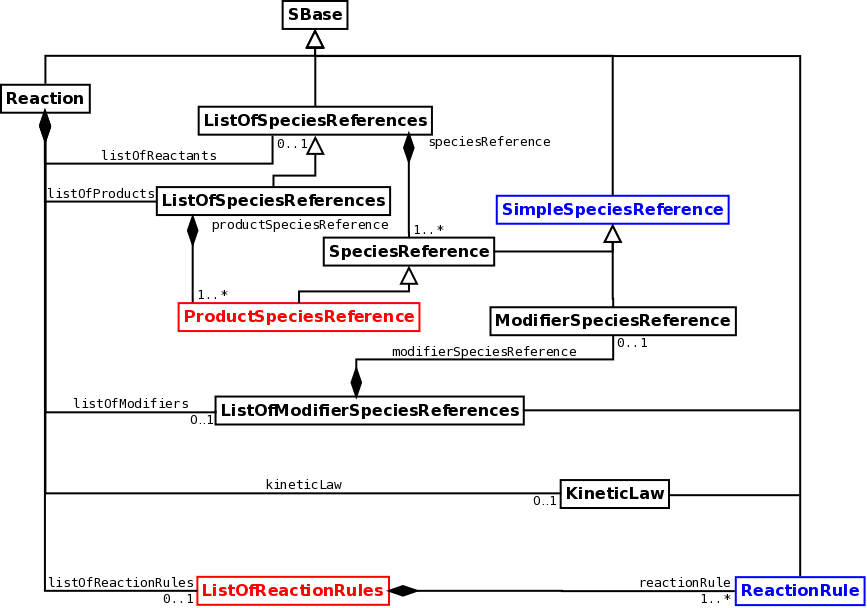
\includegraphics[scale=0.3]{./figs/pngs/ReactionGeneral.png}
\caption{\class{Reaction} and all the associated classes of \multiVone.}
\end{center}
\end{figure}

\begin{figure}[h!]
\begin{center}
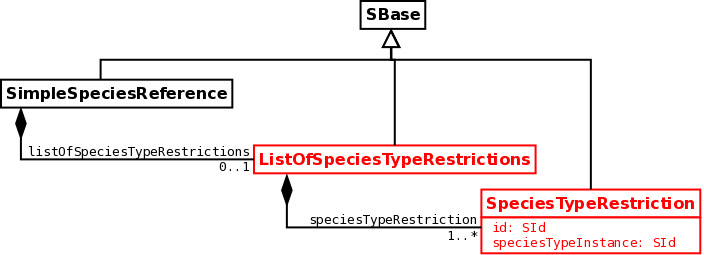
\includegraphics[scale=0.3]{./figs/pngs/SimpleSpeciesReferenceGeneral.png}
\caption{\class{SimpleSpeciesReference} and all the associated classes of \multiVone.}
\end{center}
\end{figure}

A reaction rule applies when a list of conditions is fulfiled by the reacting species, and a reaction rule produces outcomes described in a list of results. Reaction rules must not produce mass or cause unexplained disappearance of it. In other words, once the various selections are applied, what is on the left should be on the right. In order to ensure that, what is not explicitely represented must be left untouched by the reactions. 

\[*-A + B \rightarrow *-A-B\]

Can represent:

\[C-A + B \rightarrow C-A-B\]

or

\[D-A + B \rightarrow D-A-B\]

But not:

\[C-A + B \rightarrow D-A-B\]

Such a complex reaction must be explicitly described if needed.

\begin{figure}[h!]
\begin{center}
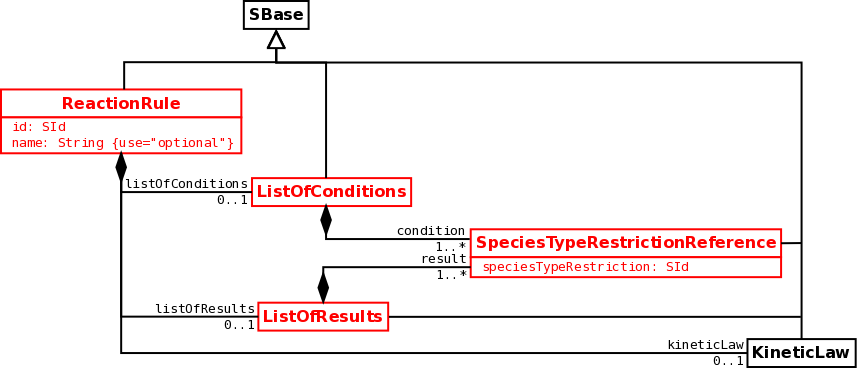
\includegraphics[scale=0.3]{./figs/pngs/ReactionRuleGeneral.png}
\caption{\class{ReactionRule} and all the associated classes of \multiVone.}
\end{center}
\end{figure}

\subsection{Reaction}

In order to encode the structures needed to propose alternative kinetic laws selected based on the state and connectivity of involved partners, we extend the element \class{Reaction} of \sbmlLthreeVone core by linking it to a list of \class{ReactionRule}s.

\begin{figure}[H]
\begin{center}
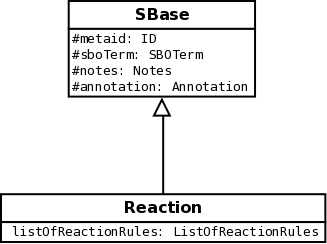
\includegraphics[scale=0.3]{figs/pngs/ReactionClass.png} 
\caption{Definition of the extended version of \class{Reaction} and its relation with \class{SBase}.}
\label{fig:ReactionClass}
\end{center}
\end{figure}

\begin{example}  
<reaction id="react" reversible="false" fast="false"
          xmlns:multi="http://www.sbml.org/sbml/level3/version1/multi/version1"> 
  <listOfReactants>
    <!-- some reactants -->
  </listOfReactants>
  <listOfProducts>
    <!-- some products -->
  <kineticLaw />
  <multi:listOfReactionRules>
    <!-- some reaction rules-->
  </multi:listOfReactionRules>
</reaction>
\end{example}

\subsection{SimpleSpeciesReference}

In order to decide which kinetic law to choose, one needs to have a list of the necessary states and connectivities for the partners involved. This is done by linking the \class{SimpleSpeciesReference} of \sbmlLthreeVone core to a list of \class{SpeciesTypeRestriction}s. There can be any number of \class{SpeciesTypeRestriction}s per \class{SimpleSpeciesReference}. They always represent alternatives, and only one can be used per \class{ReactionRule}. However, if one wants to discriminate between two instances of the same \class{Species} involved in the same \class{ReactionRule} but with different roles in the reaction, one must create two \class{SimpleSpeciesReference}s pointing to the same \class{Species}.

\begin{figure}[H]
\begin{center}
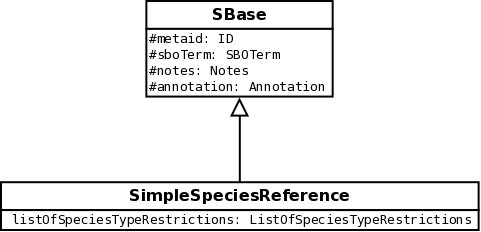
\includegraphics[scale=0.3]{figs/pngs/SimpleSpeciesReferenceClass.png} 
\caption{Definition of the extended version of \class{SimpleSpeciesReference} and its relation with \class{SBase}.}
\label{fig:SimpleSpeciesReferenceClass}
\end{center}
\end{figure}

\begin{example}
<speciesReference species="species1" stoichiometry="1"
                  xmlns:multi="http://www.sbml.org/sbml/level3/version1/multi/version1">
  <multi:listOfSpeciesTypeRestriction>
    <!-- some species type restrictions -->
  </multi:listOfSpeciesTypeRestriction>
</speciesReference>  
\end{example}

\subsection{ProductSpeciesReference}

In the cases where several instances of the same molecule are use in a reaction, we must explicit the correspondence between the reactants in the product. Otherwise, the following reactions will be selected by the same reaction rule:

\[A1-P + A2 \rightarrow A1 + A2-P\]

\[A1-P + A2 \rightarrow A1-P + A2\]

In order to do so, we create a new element \class{ProductSpeciesReference} that inherits from \class{SimpleSpeciesReference}. The element carries an attribute \attribute{correspondingReactant} that precises from which reactant instance the product originates. In an agent-based approach, this would apply to each 
molecule, while in a population-based framework, this would apply to pools. 

\begin{figure}[H]
\begin{center}
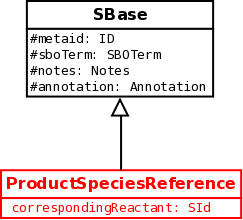
\includegraphics[scale=0.3]{figs/pngs/ProductSpeciesReferenceClass.png} 
\caption{Definition of the extended version of \class{ProductSpeciesReference} and its relation with \class{SBase}.}
\label{fig:ProductSpeciesReferenceClass}
\end{center}
\end{figure}

\begin{example}
<listOfReactants>
  <speciesReference id="R1" species="species1" stoichiometry="1"/>
  <speciesReference id="R2" species="species1" stoichiometry="1"/>
</listOfReactants>
<listOfProducts>
  <multi:productSpeciesReference species="species1" stoichiometry="1"
                xmlns:multi="http://www.sbml.org/sbml/level3/version1/multi/version1"
                multi:correspondingReactant="R1" />
  <multi:productSpeciesReference species="species1" stoichiometry="1"
                xmlns:multi="http://www.sbml.org/sbml/level3/version1/multi/version1"
                multi:correspondingReactant="R2" />
</listOfProducts>
\end{example}

\subsection{SpeciesTypeRestriction}

A \class{SpeciesTypeRestriction} points to a \class{SpeciesTypeInstances}, and creates a conditional species reference. Those various \class{SpeciesTypeRestriction}s can then be used to decide on the \class{ReactionRule} to use, and which \class{Result}s to produce. As all elements derived from \class{SBase}, it can link to \class{Notes} and \class{Annotation}, and carry a \attribute{metaid}, and an \attribute{sboTerm}.

\begin{figure}[H]
\begin{center}
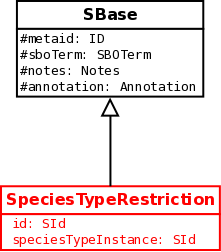
\includegraphics[scale=0.3]{figs/pngs/SpeciesTypeRestrictionClass.png} 
\caption{Definition of \class{SpeciesTypeRestriction} and its relation with \class{SBase}.}
\label{fig:SpeciesTypeRestrictionClass}
\end{center}
\end{figure}

\begin{example}
<multi:speciesTypeRestriction multi:id="speciesRest1" 
                   multi:speciesTypeInstance="speciesTypeInstance1" 
                   xmlns:multi="http://www.sbml.org/sbml/level3/version1/multi/version1"/>
\end{example}

\subsection{ReactionRule}

The \class{ReactionRule} element is used to describe a process that is dependent on states or connectivity. As all elements derived from \class{SBase}, it can link to \class{Notes} and \class{Annotation}, and carry a \attribute{metaid}, and an \attribute{sboTerm}. A \class{ReactionRule} applies when the conditions described in a \class{ListOfConditions} are fulfilled. The \class{ReactionRule} replaces the the regular \class{Reaction}. The effect of a \class{ReactionRule} is described by a \class{ListOfResults}. 

\begin{figure}[H]
\begin{center}
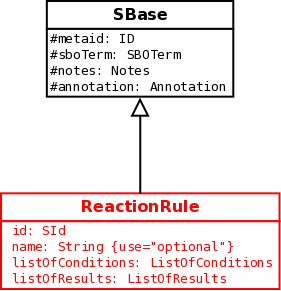
\includegraphics[scale=0.3]{figs/pngs/ReactionRuleClass.png} 
\caption{Definition of \class{ReactionRule} and its relation with \class{SBase}.}
\label{fig:ReactionRuleClass}
\end{center}
\end{figure}

\begin{example}
<multi:reactionRule multi:id="bindingNonPhospho"
         xmlns:multi="http://www.sbml.org/sbml/level3/version1/multi/version1" >
  <multi:listOfConditions>
    <!-- some conditions for the rule to be used-->
  </multi:listOfConditions>
  <multi:listOfResults>
    <!-- some results of the application of the rule -->
  </multi:listOfResults>
  <kineticLaw />
</multi:reactionRule>
\end{example}

\subsection{SpeciesTypeRestrictionReference}

In order to precise the conditions for a reaction rule to apply, and describe the results to obtain, a \class{SpeciesTypeRestrictionReference} points to a species type restriction using the attribute \attribute{speciesTypeRestriction}. As all elements derived from \class{SBase}, it can link to \class{Notes} and \class{Annotation}, and carry a \attribute{metaid}, and an \attribute{sboTerm}. The \class{SpeciesTypeRestriction}s used to decide if a rule applies are called in \class{ListOfConditions}. The \class{SpeciesTypeRestriction}s used to decide if the result of a rule are called in \class{ListOfResults}.

\begin{figure}[H]
\begin{center}
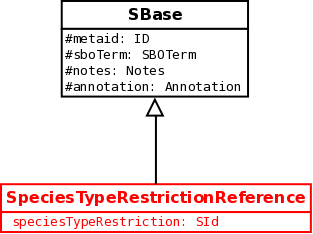
\includegraphics[scale=0.3]{figs/pngs/SpeciesTypeRestrictionReferenceClass.png} 
\caption{Definition of \class{SpeciesTypeRestrictionReference} and its relation with \class{SBase}.}
\label{fig:ConditionClass}
\end{center}
\end{figure}

\begin{example}
<multi:speciesTypeRestrictionReference multi:speciesTypeRestriction="freeRnonP"
          xmlns:multi="http://www.sbml.org/sbml/level3/version1/multi/version1" />
\end{example}

\subsection{ReactionRule -specific KineticLaw}

A \class{ReactionRule} optionally contains a \class{KineticLaw}. If the conditions apply, this \class{KineticLaw} is used to compute the results instead of the one contained in the reaction element of \sbmlLthreeVone. Note that the semantic of the model stripped of all information belonging to \multiVone may be understood in very different ways if the reaction does not contains a kineticLaw or contains an empty one. In the former case, stripping the species restrictions could means that the reaction always occurs, while in the latter, the reaction would have a flux of 0, effectively never happening. In the kinetic law of a reaction rule, the quantities of species are represented by the \attribute{id} of the \class{SpeciesTypeRestriction}s, and not the \attribute{id} of the  \class{Species}. This allows for multi-component reactions, where instances of the same species are playing different roles.

\subsection{Complete example of a reaction with reaction rules}

The following example describes a binding reaction that takes place ten times faster on the phosphorylated receptor than on the non-phosphorylated one.

\begin{example}
<reaction id="receptLigBinding" reversible="false" fast="false"> 
  <listOfReactants>
    <speciesReference id="spRef_Rec" species="receptor" stoichiometry="1">
      <multi:listOfSpeciesRestriction>
        <multi:speciesRestriction multi:id="restriction1" 
                                  multi:speciesTypeInstance="receptorNP" />
        <multi:speciesRestriction multi:id="restriction2"
                                  multi:speciesTypeInstance="receptorP" />
      </multi:listOfSpeciesRestriction>
    </speciesReference>
    <speciesReference species="ligand" stoichiometry="1" />
  </listOfReactants>
  <listOfProducts>
    <productSpeciesReference species="receptor" stoichiometry="1" 
                      correspondingReactant="spRef_Rec">
      <multi:listOfSpeciesRestriction>
        <multi:speciesRestriction multi:id="restriction3"
                                  multi:speciesTypeInstance="receptorBound" />
      </multi:listOfSpeciesRestriction>
    </productSpeciesReference>
  </listOfProducts>
  <kineticLaw>
    <math xmlns="http://www.w3.org/1998/Math/MathML" />
  </kineticLaw>
  <multi:listOfReactionRules>
    <multi:reactionRule multi:id="reactionRule1">
      <multi:listOfConditions>
        <multi:speciesTypeRestrictionReference multi:speciesTypeRestriction="restriction1"/>
      </multi:listOfConditions>
      <multi:listOfResults>
        <multi:speciesTypeRestrictionReference multi:speciesTypeRestriction="restriction3"/>
      </multi:listOfResults>
      <kineticLaw>
        <math xmlns="http://www.w3.org/1998/Math/MathML" >
          <ci> parameter1 </ci>
        </math>
        <listOfLocalParameters>
          <localParameter id="parameter1" value="1">
        </listOfLocalParameters>
      </kineticLaw>
    </multi:reactionRule>
    <multi:reactionRule multi:id="reactionRule2">
      <multi:listOfConditions>
        <multi:speciesTypeRestrictionReference multi:speciesTypeRestriction="restriction2"/>
      </multi:listOfConditions>
      <multi:listOfResults>
        <multi:speciesTypeRestrictionReference multi:speciesTypeRestriction="restriction3"/>
      </multi:listOfResults>
      <kineticLaw>
        <math xmlns="http://www.w3.org/1998/Math/MathML" >
          <ci> parameter2 </ci>
        </math>
        <listOfLocalParameters>
          <localParameter id="parameter2" value="10">
        </listOfLocalParameters>
      </kineticLaw>
    </multi:reactionRule>
  </multi:listOfReactionRules>
</reaction>
\end{example}
